La morphologie mathématique pour les images à niveaux a été développée après la morphologie binaire, dans le but de généraliser cette technique aux images fonctionnelles \cite{Haralick_1987, Serra_1992}. Dans ce cas plus général, les images et éléments structurants sont considérés comme des applications sur une partie de $E$ à valeurs dans une partie d'un autre ensemble tel que $\mathbb{Z}$ ou $\mathbb{R}$ pour les images à tons de gris, $\mathbb{Z}^3$ ou $\mathbb{R}^3$ pour les images en couleurs, ou tout autre ensemble construit comme groupe pour l'addition. \\

\vspace{-1.6mm}
Les opérations fondamentales de la morphologie mathématique sont l'érosion et la dilatation. On étudiera par la suite uniquement le cas des images à tons de gris. \\

\vspace{-1.6mm}
\noindent L'image fonctionnelle est notée $f: E \rightarrow G$. L'élément structurant est, comme l'image, une fonction notée $b: E \rightarrow G$, avec $G$ groupe pour l'addition ($\mathbb{Z}$ ou $\mathbb{R}$).

\vspace{0.4cm}
\begin{itemize}[leftmargin=*]
    \item[$\bullet$] L'érosion $\epsilon_b(f)$ de $f$ par $b$ est l'image $\epsilon_b(f) : E \rightarrow G$ définie pour tout $x \in E$ par : 
    \begin{equation}
        \epsilon_b(f)(x) = (f \ominus b)(x) = \min_{y \in E} \left \{ \, f(y) - b(y-x) \, \right \}
        \label{grey_erosion}
    \end{equation}
\end{itemize}
\vspace{0cm}
\begin{itemize}[leftmargin=*]
    \item[$\bullet$] La dilatation $\delta_b(f)$ de $f$ par $b$ est, quant à elle, l'image définie pour tout $x \in E$ par : 
    \begin{equation}
        \delta_b(f)(x) = (f \oplus b)(x) = \max_{y \in E} \left \{ \, f(y) + b(x-y) \, \right \}
        \label{grey_dilation}
    \end{equation}
\end{itemize}

\noindent Les processus d'érosion et de dilatation sont tous deux illustrés sur un exemple fig. \ref{fig:morpho_grey_operations_example}. \\

\vspace{-1.6mm}
On définit l'ouverture et la fermeture par les mêmes combinaisons entre l'érosion et la dilatation que dans la morphologie binaire. L'ouverture fonctionnelle $\circ$ est ainsi définie par : $\gamma_b(f) = \delta_b(\epsilon_b(f))$ ; et la fermeture fonctionnelle $\bullet$ par : $\phi_b(f) = \epsilon_b(\delta_b(f))$.  Il en est de même pour le gradient morphologique : $\text{grad}_b(f)=\delta_b(f)-\epsilon_b(f)$. \\

\vspace{-1.6mm}
Un lien direct entre la morphologie en niveaux de gris et la morphologie binaire peut se faire. Soit $B \subset E$ le support de l'élément structurant tel que défini dans la morphologie binaire. En définissant b comme fonction structurante plate telle que, pour tout $x \in E$ :

\vspace{-3.0mm}
\begin{center}
    $b(x) = \left \{    \begin{array}{rcl} 0 & \hspace{3.2mm} \text{si} \hspace{1.5mm} x \in B \\ -\infty & \text{sinon} \end{array}     \right.$  ,
\end{center}

\vspace{1.2mm}
\noindent les formules \ref{grey_erosion} et \ref{grey_dilation} permettent à la morphologie en niveaux de gris d'avoir le même comportement que la morphologie binaire, pour des images binaires définies comme fonctions sur E à valeurs dans $\{0,1\}$.

\vspace{2.5mm}
\noindent La formule de l'érosion devient alors : \hspace{4mm} $\epsilon_b(f)(x) = \min_{y \in B_{x}} \left \{ \, f(y) \, \right \}$

\noindent Et celle de la dilatation devient ainsi : \hspace{5mm} $\delta_b(f)(x) = \max_{y \in \breve{B}_{x}} \left \{ \, f(y) \, \right \}$

\vspace{2.5mm}
\noindent $\min_{y \in B_{x}} \left \{ \, f(y) \, \right \}$ correspond à l'inclusion de $B_x$ dans les objets de l'image $f$ au point $x$, et $\max_{y \in \breve{B}_{x}} \left \{ \, f(y) \, \right \}$ à la non vacuité de l'intersection entre $\breve{B}_x$ et les objets de $f$ en $x$.


\newpage

%figure
\vspace{2.0mm}
\begin{figure}[ht]
  \begin{center}
      \subfigure[Processus d'érosion évalué en un point $x$]{
          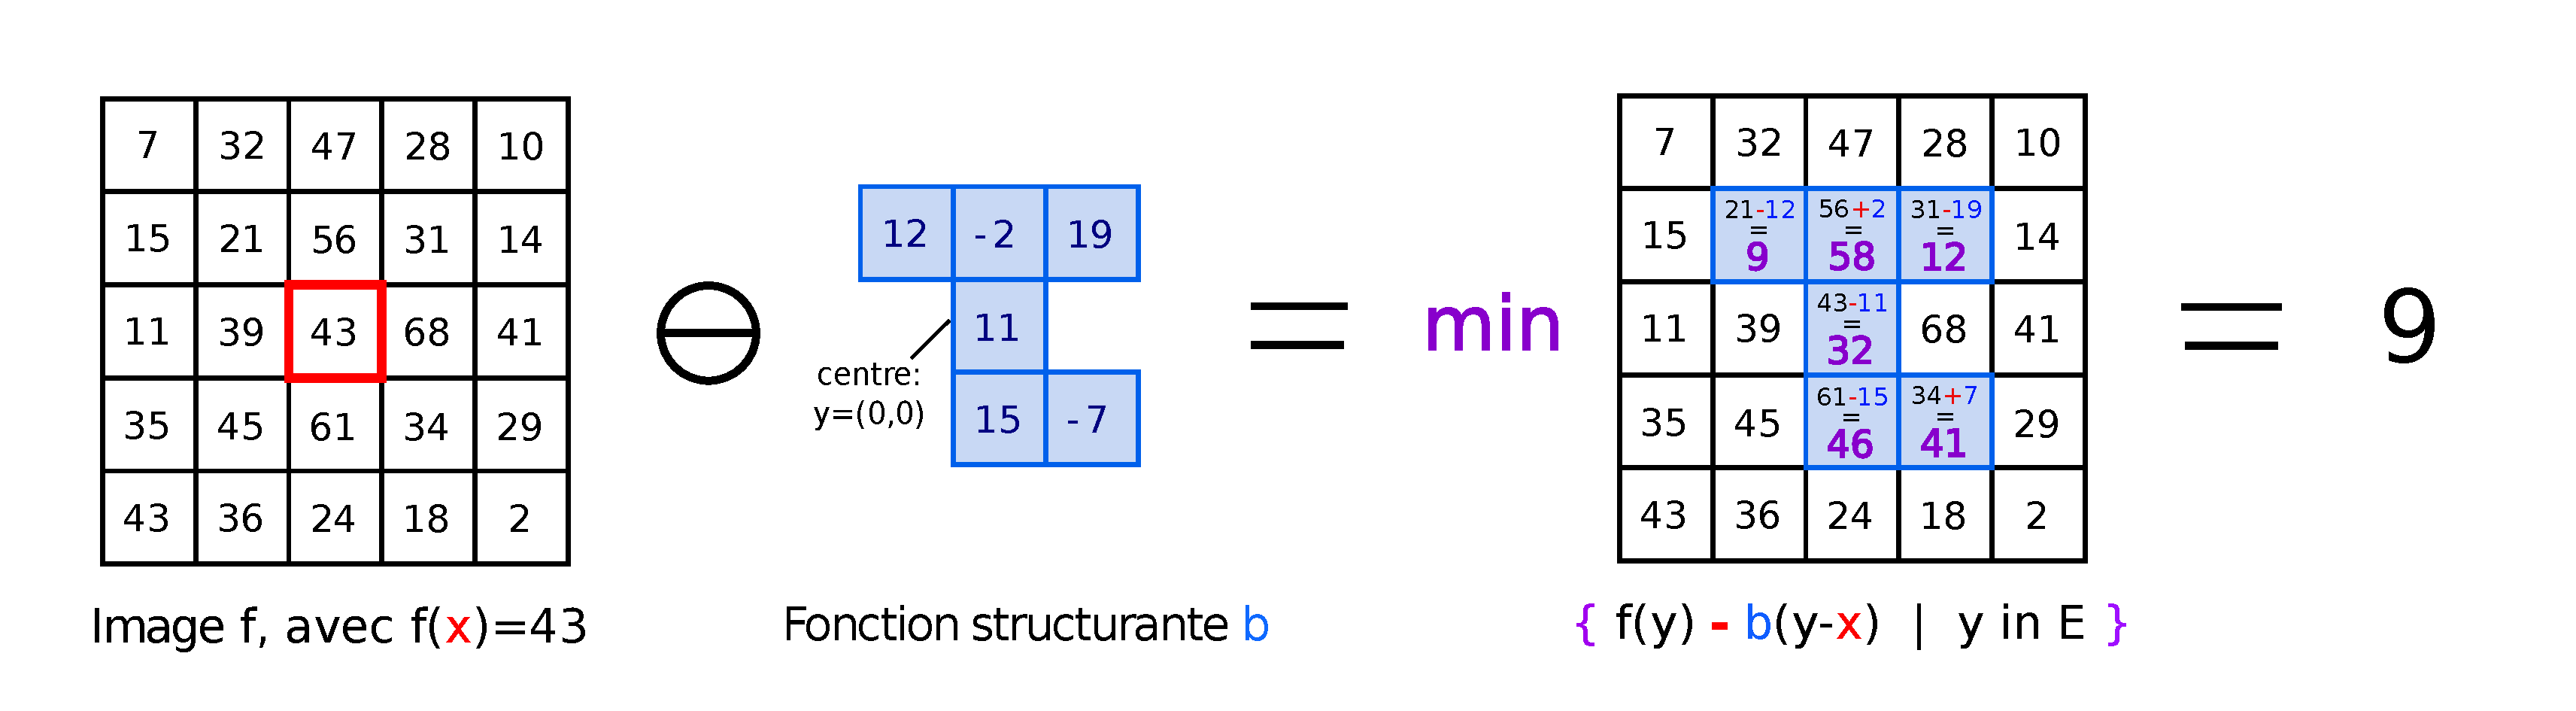
\includegraphics[width=1.00\textwidth]{parts/2-etat_de_lart/A-operateurs_morphologiques_classiques/figures/grey_erosion.pdf}
          \label{fig:sus1}}\hfill
      \subfigure[Processus de dilatation évalué au même point $x$]{
          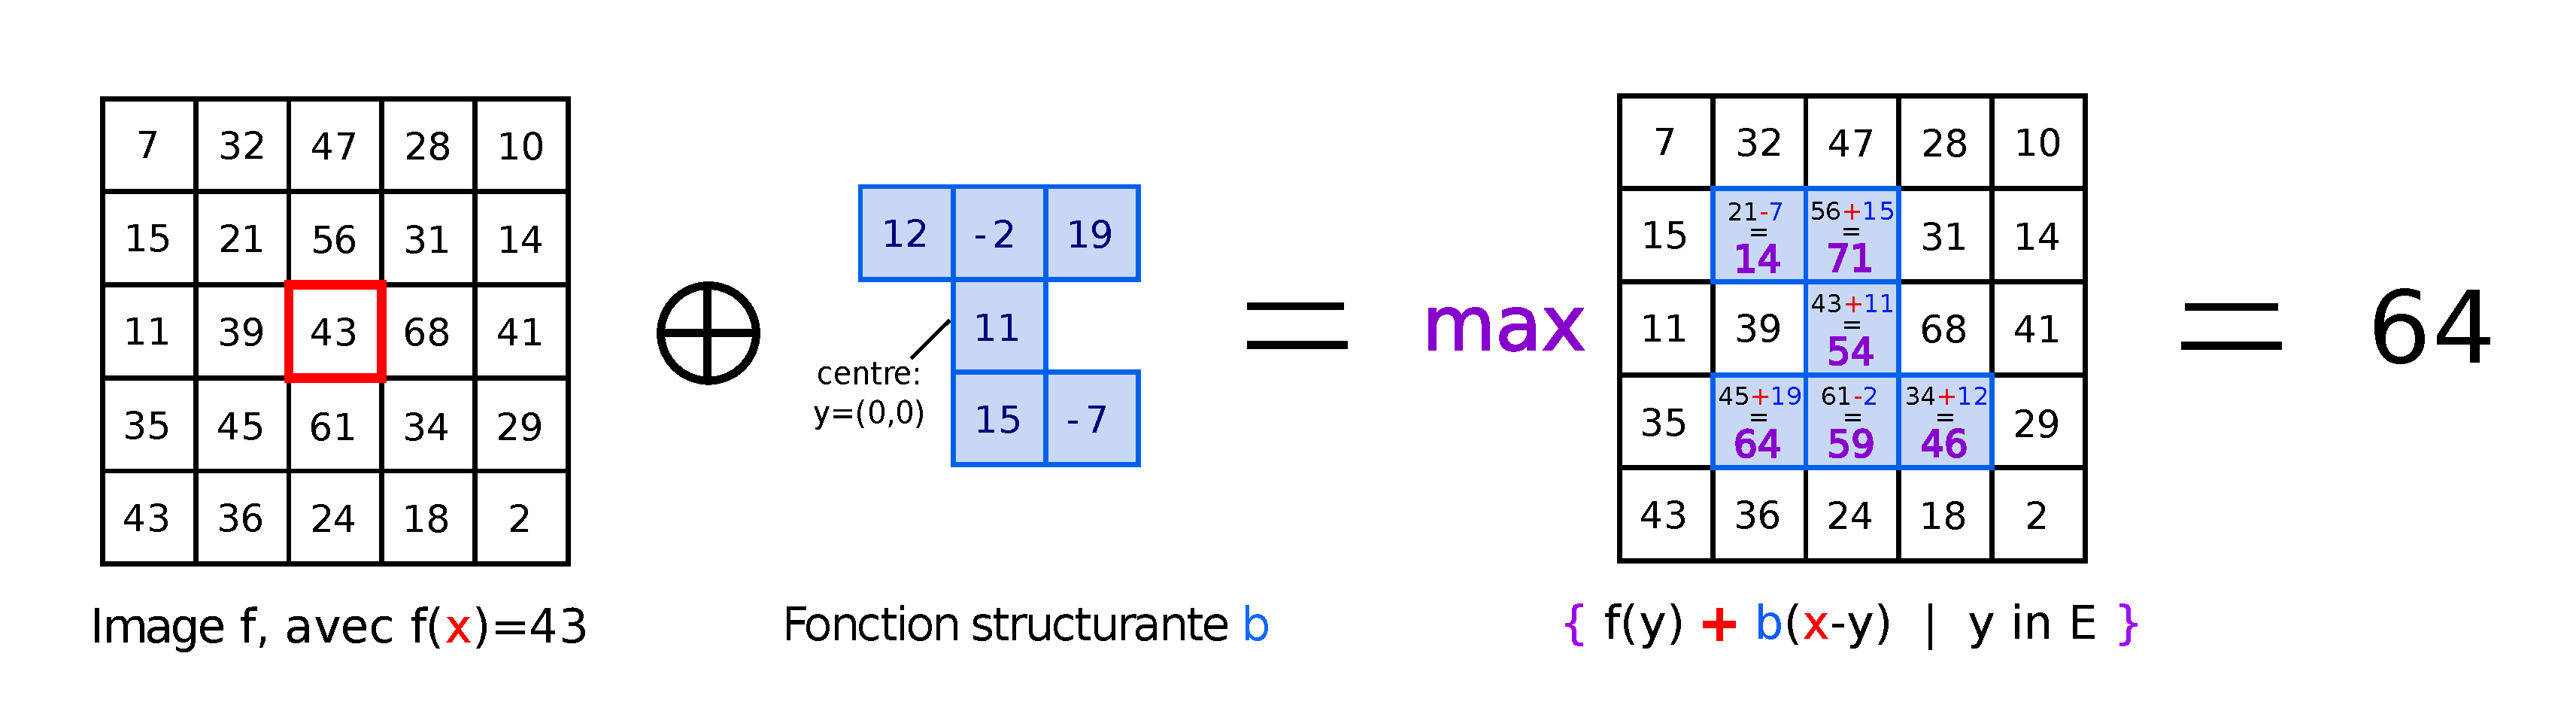
\includegraphics[width=1.00\linewidth]{parts/2-etat_de_lart/A-operateurs_morphologiques_classiques/figures/grey_dilation.pdf}
          \label{fig:sus2}}
    \caption{ \centering Exemple du processus de l'érosion $\ominus$ \ref{fig:sus1} et de celui de la dilatation $\oplus$ \ref{fig:sus2} sur une image $f$ en niveaux de gris, en un point $x \in \mathbb{Z}^2$, et par un élément structurant $b$.}
    \label{fig:morpho_grey_operations_example}
  \end{center}
\end{figure}

\vspace{1.0mm}
\noindent \textbf{Remarque pour la suite :} \\

\vspace{-0.6mm}
En morphologie mathématique, que ce soit en binaire ou en niveau de gris, la dilatation considère la symétrie $\breve{b}=-b$ de l'élément structurant $b$, contrairement à l'érosion qui considère simplement $b$ \cite{Haralick_1987}. En niveaux de gris, cela est illustré par l'inversion de $x$ avec $y$, en argument de l'élément structurant $b$, entre l'érosion et la dilatation. Voir les formules précédentes, ainsi que l'illustration fig. \ref{fig:morpho_grey_operations_example}. Il s'agit d'un élément important dans la suite de ce rapport, où les différentes formules d'appriximation de ces opérations morphologiques considèrent soit uniquement $b$ soit uniquement sa symétrique $\breve{b}$ pour ces deux opérations à la fois, afin de conserver la continuité des formules lors du passage d'un effet d'érosion à un effet de dilatation, et inversement. \\

\vspace{-1.6mm}
\noindent De plus, dans la morphologie en niveaux de gris, la seconde différence de construction entre l'ensemble affecté au min de l'érosion et celui affecté au max de la dilatation, est le signe devant l'élément structurant $b$. Voir formules associées \ref{grey_erosion} et \ref{grey_dilation}. Cette seconde différence joue également un rôle important pour la suite, dans la définition des formules d'approximation de ces opérateurs morphologiques. 

\vfill

%%% ASPECT FONCTIONNEL (on considère des fonctions d'un sous-ensemble de Z² dans un sous-ensemble d'un autre groupe, genre R ou Z)